To accomplish our goal of detecting whether a face is present in one given image, we need to first explain the methods that will be used. Let us, therefore, look into Machine Learning (\textit{ML}) from a theoretical perspective. We will address three main points in this chapter: the problems ML tries to solve, what a Convolutional Neural Network (\textit{CNN}) consists of, and, lastly, how such a theoretical contraption is relevant for our application - we will discuss, amongst others, training, parameters, hyperparameters, and optimization. A thorough, textbook-like, explanation is not intended. Instead, the focus will be on offering a brief overview of the key concepts.
\section{Machine Learning}
As Tom Mitchell put it in his 1997 book, \textit{Machine Learning is the study of computer algorithms that improve automatically through experience}. \cite{mitchell_ml} Let us expand on this definition: we want to have an algorithm, that \textit{learns} from \textit{data} and translates that experience into a mathematical model, which is used to make predictions or decisions, without the system designer having explicitly programmed a solution to the problem beforehand. \cite{genetic_book_96} \par

Let us first define some key terms:
\begin{itemize}
    \item \textbf{Dataset}: this refers to a collection of data points, either labeled or not, belonging to different classes and categories of objects, which our ML model is to learn about. A sample is offered in \textit{Figure \ref{margot_robbie_9}};
    \begin{figure}
        \centering
        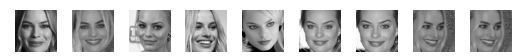
\includegraphics{images/margot_robbie_good.png}
        \caption{Sample images from a training dataset, showing Margot Robbie. The cropping around the face is very tight in this example. The amount of padding can and often does influence model performance.}
        \label{margot_robbie_9}
    \end{figure}
    \item \textbf{Training}: also known as \textit{fitting}, this is the iterative process of \textit{learning} from the given data and the different classes of training will be discussed below. After a network has finished training on data, its state becomes permanent - it becomes what is known as a \textit{frozen} tensor;
    \item \textbf{Inference}: this is the part that comes \textit{after} training, and refers to using the ML model on actual data, to draw conclusions and accomplish something in the real world. For instance, using a face detector to look for faces in an image is inference - an image is given as input, mathematical operations from the oriented graph of the neural network are applied to that image tensor, and an output is eventually computed from mathematically \textit{combining} these two objects.
\end{itemize}



\subsection{Classes of Learning and ML Algorithms}
There are many different classes of Machine Learning. They can generally be broken up by type of training, or by desired outcome. Let us look at ML from the first perspective. There are, in essence, three types of learning: supervised, unsupervised, and reinforcement learning \cite{DBLP:journals/corr/cs-AI-9605103}. \textit{Supervised learning} means that we train the network in a controlled, procedural manner, usually offering data and \textit{feedback} at each training step. This translates to using labeled datasets - each data point has something similar to a \textit{name tag}. Thus, the neural network learns where that data point belongs. \textit{Unsupervised learning} refers to the algorithm analyzing data on an \textit{as is} basis, observing features and drawing its own conclusions from it, without direct feedback from the trainer - this category of systems is following patterns and trends in the data, instead of relying on a third party trainer, of which there is none, in contrast to supervised learning methods. This usually implies that the computer will try to learn a complete statistical overview of the data to understand it. The main difference between the two can be formulated as follows: supervised learning means that we study different instances of \textit{x}, each with a known \textit{y}, and learn to predict unknown \textit{y's} for new \textit{x's}; unsupervised learning means we observe some interesting features and probabilistic properties of \textit{x} and try to determine, as Goodfellow et al have it, its probability distribution \textit{p(x)}. The final class is \textit{Reinforcement Learning}, which, as the name suggests, keeps on learning in a sustained manner. This is a direct result of the fact that, in comparison to supervised and unsupervised learning - where training is completely separated from inference - in reinforcement learning, we don't have such a strict limit between the two. Instead, the algorithm keeps on learning while being used, and from new data. This also leads into the next big difference with reinforcement learning, namely that it is primarily used for dynamic systems. This can be useful, for instance, in places where there is a \textit{feedback loop}, such as in control theory-related problems and automation tasks. We will not go into more detail on reinforcement learning techniques. \par
Let us now analyze ML algorithms from the second perspective - the desired outcome. Here, we can have procedures to make predictions (regression), to detect and analyze patterns, or divide the data according to commonalities (cluster analysis), to classify one given input into one of several classes (classification), and lastly, to derive and \textit{distill} features from data thorough feature reduction. This thesis will focus on classification algorithms only. This class of ML can generally leverage all three kinds of learning - supervised (for instance, \textit{Naive Bayes}), unsupervised (for instance, \textit{Support Vector Machines - SVM} or \textit{Random Forests}, which both also use supervised learning) and reinforcement (generally, only \textit{Neural Networks} can use all 3 types of learning) \cite{Goodfellow-et-al-2016}. An overview, with more examples, can be found in \textit{Table \ref{classes_ml}}.

\begin{table}
    \centering
    \begin{tabular}{|l||*{3}{c}|}\hline
        \backslashbox{Task}{Class}
        &\makebox[3em]{Supervised}&\makebox[4em]{(Partially) Unsupervised}&\makebox[4em]{Reinforcement}
        \\\hline\hline
        Regression & Linear\&Logistic & Conditional GAN &\\\hline
        Cluster Analysis & & K-Means\&Anomaly Detect. &\\\hline
        Classification & Naive Bayes & SVM/SVC  \cite{svc_paper} & Neural Networks*  \\\hline
        Feature Reduction & & PCA&\\\hline
    \end{tabular}
    \caption{Classes of Machine Learning and their related tasks. Neural Networks can use more than one learning technique during their training, or just any single one of the 3. \cite{reinforcement_nn} Conditional GAN's can be used to generate new data, such as new images, whereas linear and logistic regression are older, less sophisticated techniques, used to approximate functions. \cite{GAN_regression} Naive Bayes is a name for problem-solving techniques based on statistical analysis. SVM's can work as both supervised and unsupervised learners - in which case the method will be called \textit{support vector clustering - SVC}. This table only has the intention to offer a very brief overview.}.
    \label{classes_ml}
\end{table}
However, for our application, let us focus on supervised learning with Neural Networks. 

\section{Deep, Convolutional Neural Networks}
Neural Networks are mathematical objects modelled after \textit{brains} (human or animal) \cite{Goodfellow-et-al-2016}. The main focus is that they use \textit{connections} to make sense of data. However, let us not expect that this anatomical analogy will go any further, since we do not intend to discuss neurology or the cognition mechanisms of living creatures. The term \textit{deep} is an indication of the fact that the \textit{insides} of these mathematical representations are \textit{hidden} from view, whereas the term \textit{convolutional} is a reference to the fact that the type of networks we will discuss below employ at least one \textit{convolutional layer}. A visual representation is given in \textit{ Figure \ref{deep_NN_fig}}.

\subsection{Key Terminology}
Therefore, let us continue by introducing some key terminology related to CNN's: 
\begin{itemize}
    \item \textbf{Node:} also neuron or cell, this is one unit of the neural network. It is the intersection of \textit{connection lines} inside the network, and is often a place where mathematical operations will be applied to the data.
    \item \textbf{Layer:} this is often described in literature as a level of the network \cite{Goodfellow-et-al-2016}. It can be either \textit{visible} - input and output layer - or \textit{hidden} - located inside the network, in between the two.
    \item \textbf{Input Layers:} this refers to the data being fed into the Neural Network, such as an image; it will usually have been processed into a mathematical object. For instance, inputs are often multi-dimensional matrices, or \textit{tensors}. 
    \item \textbf{Output Layers:} this represents the result that the neural network produces; for example, a multi-class classifier will deliver different percentages for each class it has to classify an object into, with each percentage representing its rate of confidence that the given input object belongs to that specific class.
    \item \textbf{Convolution:} in our case, this does not refer to the mathematical operation from Fourier Analysis. Instead, convolution refers to \textit{dragging} a filter layer across a matrix or tensor to obtain a different representation of that structure - more formally, applying a linear transformation to a tensor, which results in a different representation, that can be more useful to a computer. By \textit{different} representations, we mean new tensors, such as \textit{feature maps} or \textit{oriented gradient representations}, which help the computer more aptly visualize the trends and patterns in the data, which it can subsequently learn from. \subfile{figures/deep_nn}
    \item \textbf{Kernel:} this is the \textit{unit} of convolution; it is the \textit{window} that we drag over the input data to derive the convoluted representation out of it.
    \item \textbf{Pooling:} by this, we mean the process of \textit{summarizing} or \textit{compressing} several points into a single, new value. For instance, \textit{max-pooling} takes the maximum value from a matrix. \textit{Average-pooling} takes the mean value instead.
    \item \textbf{Weights and Biases:} these are the numerical values that the neural network learns during training, to represent an output \textit{f(x, w)} as a linear combination of the given \textit{n-dimensional} input \textit{x} and the \textit{n-dimensional} weight vector \textit{w}, plus the bias:
    \begin{equation}
        f(x, w) = x_1*w_1 + ... + x_n*w_n + b
    \end{equation}
    \item \textbf{Activation function:} Generally, this will be a Rectified Linear Unit (ReLU) for convolutional neural networks; it is used right before the output layer to eliminate negatives and deliver a result inside the correct interval - above zero. Another very popular kind of activation function is Softmax. Examples of both are presented in \textit{Figure \ref{fig:relu_softplus}}. \cite{activations}
    \begin{figure}
        \centering
        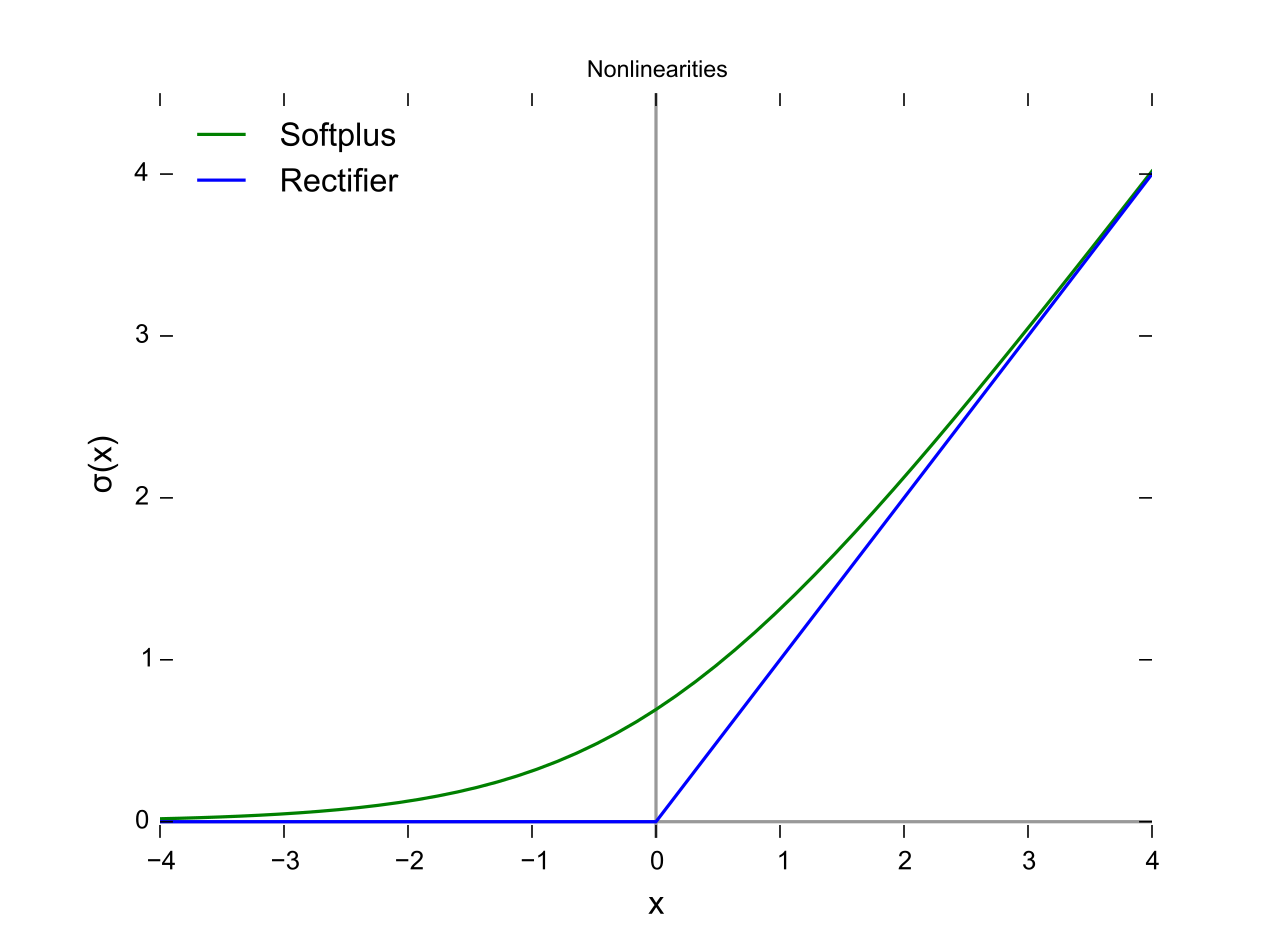
\includegraphics[width = 12 cm]{images/1280px-Rectifier_and_softplus_functions.svg.png}
        \caption{A ReLU (blue) and a Softplus (green) activation functions. Source: \cite{activations_figure}}
        \label{fig:relu_softplus}
    \end{figure}
    \item \textbf{Loss:} this refers to the \textit{penalization} given to the NN for delivering results that differ from the expected output. For instance, widely used loss-layers include \textit{sigmoid cross-entropy loss} or \textit{softmax layers}.
\end{itemize}

\subsection{On the Efficiency of the Convolution Operation}
Given the fact that our model is to run on small, embedded devices, we should not forget that convolution is, at least in its general formulation, a highly inefficient operation, from a computational resources point of view - according to Goodfellow et al, it stands on the scale of \textit{O\((n^2)\)}. Modern applications often also use parallelization to save hardware power. \cite{Goodfellow-et-al-2016}. We should also note, again, the difference between inference and training: in our case, we can only afford inefficient allocation of resources during training, but, for inference, this has to be tightly controlled, since inference must run on MCU's. We will address this problem again in the following chapters. An example for one widely used procedure is \textit{General Matrix to Matrix Multiplication - GEMM}, or \textit{im2col}. This operation implements convolution as linear matrix multiplication but arranges data differently from the standard element-wise order used when calculating per definition, to benefit from the memory access policies of computers. For instance, im2col takes advantage of data locality in RAM and, as such, increases performance, even if this comes with a memory capacity trade-off, given the relatively high amount of created redundant data. \cite{pete_warden_gemm}
A simple numerical example is given in \textit{Figure \ref{fig:convolution_ex}}. \subfile{figures/convolution}

\section{Training, Hyperparameters, and Optimization}
Let us look into the training workflow of Convolutional Neural Networks. We will discuss four \textit{parameters} - also known as \textit{hyperparameters} that should be tweaked during training to optimize performance and increase accuracy, or, formulated in a more compact, mathematical way, to minimize loss.
\begin{itemize}
    \item The number of training \textit{epochs} (repetitions) that we train the network for;
    \item The size (in number of samples) of the \textit{data batches} that we feed the neural network for every individual step of the training;
    \item The \textit{divide} between training and testing data; for instance, many applications choose to reserve around 30\% of the data for testing, while using the rest for training. It is also possible to reserve a small portion of the samples for what is known as validation - these samples will only be used for inference at the very end to more objectively evaluate the performance of the fully trained and \textit{frozen} neural network;
    \item The \textit{dropout rate}, which is the number of weights we simply delete out of the network after each training epoch to prevent overfitting.
\end{itemize}
Let us now investigate 3 other important metrics, which have a high impact on training performance.
\begin{itemize}
    \item \textit{Generalization error}: this measures the amount of \textit{guessing} a trained model would do; in other words, the more \textit{blank spots} there are in the training data, the more we can expect our model to have an erratic behavior when presented with inputs it had never seen before, during inference.
    \item \textit{Bias}: this defines the tendency of the trained model to over-perform (in terms of e.g. classification or regression accuracy) for certain categories of inputs, while delivering sub-par performance or accuracy for others.
    \item \textit{Variance}: this is the statistical \textit{diversity} of data; in other words, this will mathematically represent the scale of \textit{squared difference} we can allow our training samples to divert from their common mean. Higher variance generally means a more versatile and robust system, that can deliver better results on more varied inference inputs.
\end{itemize}

Let us now discuss \textit{underfitting} and \textit{overfitting}, which are two of the most common problems we must overcome during fitting.
\begin{itemize}
    \item \textbf{Underfitting} is the problem that arises when the training data fails to represent the model in its full complexity. This means that there will be missing features or certain intervals of the \textit{to-be-predicted function} are simply left out, and it is up to the algorithm to fill out these blank spots - often having less than ideal outcomes in terms of accuracy; the model will simply not know enough to make accurate calls. Underfitting can be caused either by simply having too little training data, in which case we need to increase the amount (and quality) of training data, or, in other cases, by an inappropriate choice of hyperparameters, such as too low of a number of training epochs, in which case the model does not have enough time to train.
    \item \textbf{Overfitting} is the exact opposite problem and it arises when the training fails to give the neural network a wide enough view of the problem for it to be able to generalize on new, real-life situations. This can also be seen as the model having focused so hard on the \textit{minutia} of the training data, that it misses the \textit{bigger picture}. Models trained in this manner will perform excellently on the training and testing data but will deliver poor results in the real-world. This is caused by either too little variance, or \textit{diversity} in the training data - alas \textit{no big picture}, or by a poor choice of hyperparameters such as batch sizes or training epochs - training for too long and with too little data in every step will likely result in overfitting.
\end{itemize}
\subfile{figures/under_overfitting}
The optimal point where we want our trained model to be is, therefore, right in the middle: neither too general nor spread out too thin, nor too specialized on the minutia of training data and \textit{missing the bigger picture}. We want it to be just rightly balanced between these two; this is where neural networks tend to perform best. This is represented in \textit{Figure \ref{fig:over_underfitting}}. What we obtain is a \textit{U-shaped} curve for the generalization error of the trained network model, represented in \textit{Figure \ref{fig:over_underfitting}}. We want our trained model to fall somewhere in the middle for optimality, as per \textit{Goodfellow et al}. \cite{Goodfellow-et-al-2016}

\section{Final Notes}
\begin{table}[]
    \centering
    \begin{tabular}{|c|c c|}\hline
        No. & \textbf{Name} & Description\\\hline
        1 & 2D Convolution & \\\hline
        2 & Activation Layer & ReLU \\\hline
        3 & 2D MaxPooling & maximum of a region \\\hline
        4 & 2D Convolution & \\\hline
        5 & Activation Layer & ReLU \\\hline
        6 & 2D MaxPooling & maximum of a region \\\hline
        7 & Flattening Layer & \\\hline
        8 & Dense Layer & fully-connected neurons\\\hline
        9 & Activation Layer & ReLU \\\hline
        10 & Dense Layer & fully-connected neurons \\\hline
        11 & Activation Layer & Softmax \\\hline
    \end{tabular}
    \caption{A classifier Convolutional Neural Network architecture}
    \label{tab:sample_net}
\end{table}
Let us reiterate the main points that have been addressed in this chapter. We started out by discussing the problem Machine Learning tries to solve, and defined ML as a mechanism that tries to correctly \textit{fit} or \textit{estimate} an unknown function, and implicitly minimize the amount of \textit{difference} there is between the \textit{estimated function} and the real, \textit{unknown function}. For our specific use case, we need a Convolutional Neural Network mechanism that can \textit{classify} the given input into one out of several given categories; the model comprises of \textit{nodes} and  \textit{layers}, representing \textit{weights} and \textit{biases}, that take an image as input and deliver percentages as outputs. After designing a model, we \textit{train} and \textit{test} it with data, evaluate its performance by certain \textit{metrics}, then change and \textit{drop} parameters accordingly, to improve its \textit{accuracy}, and \textit{minimize its loss}. A sample convolutional neural network model architecture can be seen in \textit{Table \ref{tab:sample_net}}. \par
Having now achieved a certain level of understanding of the fundamentals of Machine Learning, and Convolutional Neural Networks, we can now confidently dive into the next chapter, where we will discuss the reasons why we want to bring ML down into the embedded world of tiny devices, as well as which technical problems we encounter along the way - while proposing solutions for most of them, too. \par
